\chapter{Overview of the Approach}

This chapter gives an overview of my approach of JavaScript static analysis using the \emph{Codemodel-Rifle} framework.


\section{Refactoring the Codemodel-Rifle Framework}

Dániel Stein, creator of the Codemodel-Rifle framework, details the design of the framework in his Master's Thesis.~\cite{stein-daniel-msc} Following his thesis and my experiences with the framework, the summary of the software's architecture is the following:

\begin{itemize}
\item A source code file is to be delivered to Codemodel-Rifle via the HTTP REST API of the framework's embedded webserver as a text.
\item The framework parses the incoming source file into an AST model with Shape Security's Shift parser.
\item The framework performs scope analysis on the AST model with Shape Security's scope analyser, transforming the AST model into an ASG model.
\item The ASG model is transformed to a property graph and is stored in the framework's embedded Neo4j graph database.
\item Apart from importing a file, the framework is able to perform analyses on or visualisation of a graph stored in its database, if requested over its REST API.
\item Analysing multiple ECMAScript files are minimally supported by interconnecting related modules' subgraphs along the \emph{export} and \emph{import} ECMAScript statements, but not all use cases and combinations are implemented.
\item The result of the analyses or the visualisation is returned via the REST API in JSON or in a visual file format.
\end{itemize}

Codemodel-Rifle was notably refactored since the state of the above summarised architecture. This section introduces why refactoring was necessary, and presents the details and the results of the process.


\subsection{Open-Sourcing and Licensing Issues}

Development of the Codemodel-Rifle framework was supported by the Fault-Tolerant Systems Research Group (FTSRG) of the Budapest University of Technology and Economics. FTSRG's decision (with the support of Dániel Stein) was to open-source the framework under FTSRG's name. According to an agreement with the university, FTSRG can only release open-source code under the Eclipse Public License, version 1.0 (EPLv1)~\cite{eplv1}. As it is maintained by the FTSRG, the Codemodel-Rifle framework is required to be released under EPLv1, if open-sourced. This introduced several licensing problems.~\cite{codemodel-rifle-licensing}

The framework uses Neo4j as its internal graph data storage, and Neo4j was embedded into Codemodel-Rifle.~\cite{stein-daniel-msc} From the point of licensing, there is an important difference between \emph{using} the database \emph{via a network connection} and \emph{embedding} the database \emph{into software}. Since Neo4j's Community Edition, used by Codemodel-Rifle, is licensed under GPLv3~\cite{neo4j-licensing}, it can be used remotely via a network connection with practically any license because of the so-called \emph{application service provider loophole}~\cite{asp-loophole}, but it can not be embedded into applications which do not comply with GPLv3. As EPLv1 and GPLv3 are incompatible, Neo4j can not be embedded into the open-sourced Codemodel-Rifle.

Consequently, a necessary step was to switch from embedded Neo4j to remote Neo4j accessed via a driver. But, as native API-calls, which were extensively used by Codemodel-Rifle, can not be used with driver-accessed remote Neo4j, this caused further problems; these are subjects of the next subsections.


\subsection{Decomposing the Architecture}

Codemodel-Rifle's first architecture was a monolith. It \emph{embedded} four key modules:

\begin{itemize}
\item a Neo4j graph \textbf{database},
\item a \textbf{webserver} exposing an HTTP REST API for interactions,
\item the \textbf{core module} responsible for transforming source code into an ASG and performing analyses on the graph,
\item and \textbf{other application logic}, e.g.\ for displaying and exporting AGSs into visual file formats like PDF or PNG.
\end{itemize}

Decoupling, or minimising direct interdependencies between components is an important aspect of software engineering. If a software is decomposed into smaller components along well-defined interfaces, it becomes modular: any module's inner functioning can be changed without affecting other modules, as long as the module implements the interface it was bound to. Motivations to alter a module include performance issues, scalability efforts, or changed domain logic. Codemodel-Rifle's first architecture was well-designed for easy manual testing and seemed to be an obvious solution for creating a small-scale graph-based analysis software. However, demands like simultaneous usage of multiple users, or having dedicated hardware resources to run analysis queries over large repositories, required the Codemodel-Rifle framework to become modular to adapt.


\subsubsection{Detaching the Database}

Apart from the licensing issues detailed above, using a remote Neo4j server as a database instead of the embedded version comes with several benefits. The database can be outsourced onto a separate hardware or infrastructure: since analyses and graph maintenance can be demanding over large code repositories, providing dedicated resources for the database is an obvious solution for possible performance issues and scalability.

With a remote Neo4j database, a custom database driver can be utilised. This driver can be capable of incremental processing on the graph database level\footnote{Gábor Szárnyas is developing a graph database driver \emph{ingraph} with the goal of evaluating openCypher queries incrementally.~\cite{ingraph-github}}, or it can support testing by providing an in-memory database instance via a driver\footnote{The default configuration of the framework is to use an in-memory Neo4j database currently. This is to be detailed in the next subsection.}.

As a result of the aforementioned benefits and licensing issues, the framework was refactored to use a remote Neo4j server via a driver. This meant native API-calls were no longer possible: interacting with the database has been restricted to Cypher queries provided via the database driver. The Codemodel-Rifle framework extensively used native API-calls, so all these function calls had to be rewritten into distinct Cypher queries. As Cypher queries turned out to be notably slower than the API, when executed many queries at once, this introduced performance issues. Solutions to these issues are described in the next sections.


\subsubsection{Eliminating the Web Interface}

The framework contained an embedded Grizzly~\cite{grizzly-website} web server to expose an HTTP REST API for user interactions. This was a convenient way for manual testing and a sensible approach for operating the software in a prospective production environment as well. All communication with the Codemodel-Rifle framework (operating as a server) could be achieved via its HTTP REST API with tool like curl~\cite{curl-website} or Postman~\cite{postman-website} (in development), or with an IDE or CI plugin (in production).

For automated testing however, an HTTP REST API is inconvenient: solutions for important testing issues like exception handling and logging do not come straightforward. Since the framework is not yet intended for in-production usage at all, but is heavily under development, an architectural decision was to eliminate the web server, and focus on the core functionality: the analyses. After removing the webserver from the architecture, the in-development way to supply code repositories to the framework for analysis is via unit tests: each test has its resources shipped along with the framework's source code.


\subsubsection{Separating the Visualisation Logic into an Isolated Project}

Visualising the ASG of an imported JavaScript source code is key for getting acquainted with Codemodel-Rifle's ASG-semantics, as well as for developing new analyses. \Cref{fig:codemodel-rifle-asg} displays an example of an ASG created and visualised by Codemodel-Rifle. However, the framework does not explicitly need this feature to function as an analysis software. Therefore it was a rational step to separate the visualisation logic into an isolated project, called \emph{Codemodel-Visualization}\footnote{The project name uses US English, while this thesis aims to be in UK English.}.


\subsection{Optimising for Testing Purposes}

The framework used embedded Neo4j as a persistent storage: the project's folder contained a directory named \texttt{database}, in which the full Neo4j embedded graph database was stored. After refactoring the framework to use a remote Neo4j database server because of the aforementioned licensing issues, testing became circuitous. Using a remote Neo4j server with the framework meant the following steps were needed to run unit tests:

\begin{itemize}
\item the Neo4j Community Edition server software needed to be downloaded,
\item the designated directory to hold the database data needed to be selected,
\item the Neo4j server software needed to be started,
\item after the tests, the software needed to be stopped,
\item the database needed to be flushed between the tests to ensure the necessary level of independence of the test cases.
\end{itemize}

This process can be partially automated with scripts, but it is still not a clean way to perform automated unit tests of Codemodel-Rifle.

As a solution, Gábor Szárnyas advised to use his \emph{neo4j-drivers} project~\cite{neo4j-drivers}. The package contains wrappers and decorators for the Neo4j Java driver: with an \texttt{EmbeddedTestkitDriver} instance it is possible to use an embedded, in-memory \texttt{ImpermanentGraphDatabase} exposed as a remote database, thus being accessible via the Neo4j Java database driver. This solution is convenient for testing, since no external Neo4j database needs to be installed and run. It is also easily reconfigurable in Codemodel-Rifle by changing the framework's driver configuration in the \texttt{DbServicesManager} class only to either Neo4j's in-production Bolt driver for Java, or in the future, to an incremental driver like ingraph~\cite{ingraph-github}.


\subsection{Solutions to Speed-Related Issues: Object-Graph Mapping and the Cypher Query Builder}

Converting from embedded Neo4j to driver-accessed Neo4j, involving converting from \emph{persistent driver-accessed Neo4j} to \emph{in-memory driver-accessed Neo4j} introduced notable slowness, making testing and developing new analyses inconvenient again. \Cref{table:embedded-vs-in-memory-remote-table} shows a comparison between the duration of visualising a simple JavaScript program (the runnning example's \texttt{exporter.js} module seen on \Cref{fig:running-example-exporter}) with the old embedded, and the new in-memory driver-accessed approach.\footnote{These measurements are only for demonstrating that the framework was so slow after the necessary refactorings that it needed to be optimised even for testing. They are not aimed to be fully accurate. Evaluating the framework's performance with accurate measurements is the subject of Chapter 6.}

\begin{table}[!htb]
	\centering
	\begin{tabular}{l|cc}
		\toprule
																								& \shortstack{\textbf{embedded} \\ \textbf{database}}
																								& \shortstack{\textbf{in-memory} \\ \textbf{driver-accessed database}}
																								\\
		\midrule
		\textbf{importing, transforming, storing}   &   82ms     &   14816ms    \\
		\textbf{visualization}                      &   1832ms   &   2456ms    \\
		\midrule
		\textbf{total}                              &   1914ms   &   17272ms   \\
		\bottomrule
	\end{tabular}

	\caption{Speed comparison between the two database approach}
	\label{table:embedded-vs-in-memory-remote-table}
\end{table}

Seeing measurement results in \Cref{table:embedded-vs-in-memory-remote-table}, it was necessary to optimise the framework's performance for the in-memory driver-accessed database scenario, because extensive testing would not have been possible with such slowness. Apart from testing, optimisations will benefit the in-production performance as well, since the two environments share the same interface: in both scenario, the database is accessed via a Neo4j driver. Ideally, the optimisations should be configurable to adapt to both the testing and the production environment. In the following paragraphs, I will summarise the optimisations I performed on the Codemodel-Rifle framework.

In Dániel Stein's implementation~\cite{stein-daniel-msc}, translating the ASG model to the property graph model happens simultaneously with actually storing the property graph model in the database. If an element of the ASG model has been successfully translated into the property graph model, it is stored in the database immediately. This can be optimised: by creating a property graph model stored in Java objects, and then implementing a storage logic to perform saving the objects into the database, the operative parameters of the storage logic can be optimised directly to the currently used database driver.

\subsubsection{Creating a specialised Object-Graph Mapping (OGM) Layer}

Importing a repository can be summarised by two types of database-level action:

\begin{enumerate}
\item The ASG \emph{nodes get created} as Neo4j property graph nodes.
\item The ASG \emph{relations get set} as Neo4j property graph relations.
\end{enumerate}

Therefore, a mapping layer basically needs to translate two object types: \emph{ASG nodes} and \emph{ASG relations}. I mapped these two object types with the \texttt{AsgNode} and \texttt{AsgRelation} Java classes. An \texttt{AsgNode} stores its properties in a \texttt{HashMap}, and its labels and relations in two separate \texttt{List} members. An \texttt{AsgRelation} has a \emph{fromNode}, a \emph{toNode}, and a \emph{relationshipLabel} member. Storing relationship properties was omitted, since the Codemodel-Rifle framework semantics does not contain relationship properties.

Identifying nodes is achieved with a universally unique identifier (UUID), instead of the earlier approach of using Neo4j's discouraged \texttt{id()} function to get the nodes' built-in identifier. Each \texttt{AsgNode} object has an \texttt{id} member, which contains a value generated using the \texttt{java.util.UUID} package. The \texttt{id} member gets automatically translated into the property graph as well as all other properties. With a mapping layer like the above, it is possible to customise the procedure of storing the model in the database e.g.\ by optimising query granularity.


\subsubsection{The Cypher Query Builder}

A main bottleneck identified with the \texttt{ImpermanentGraphDatabase} interface of the \texttt{EmbeddedTestkitDriver} was the speed of parsing queries. Since the example presented in \Cref{table:embedded-vs-in-memory-remote-table} requires $201$ property graph nodes and $340$ relationships to be created, it normally requires $541$ distinct Cypher queries to be run. If multiple distinct queries are merged into one, it increases speed with nearly 50\% in some cases. Accordingly, it is a reasonable step to implement a configurable, specialised query builder, which manages storing the property graph model with a coarser query-granularity (by creating multiple nodes or setting multiple relationships within one executed database query).

The implemented query builder is capable of creating Cypher queries specially for the aforementioned OGM layer, following its internal configuration about how many \emph{ASG node creation} queries and how many \emph{ASG relation setting} queries should be merged (compressed) into one. The builder assembles and prepares the queries, and then returns them in a list. Each query in the list is a compressed query according to the configuration, ready to be executed without further modifications.


\subsubsection{Refactoring the Core Logic to Utilise the OGM and the Query Builder}

After implementing and testing the mapping layer and the query builder, I modified the core import logic of the framework in the \texttt{ASTScopeProcessor} class to utilise the new components. Instead of immediately storing the translated ASG model as a property graph model in the database, the processor first stores the property graph model in Java objects with my custom OGM layer. Then, benefiting from the query builder, the model is sent to the database in optimally sized chunks following the query builder's configuration.

\Cref{table:query-builder-config} shows the optimal configuration values of the query builder in testing environment (with the \texttt{EmbeddedTestkitDriver}), and in a prospective production environment (with the official Bolt driver of Neo4j) for test cases run on my computer.

\begin{table}[!htb]
	\centering
	\begin{tabular}{l|cc}
		\toprule
																								&   \textbf{testing}   &   \textbf{production}   \\
		\midrule
		\textbf{nodes created in one query}         &   16                 &   20                    \\
		\textbf{relationships set in one query}     &   1                  &   2                     \\
		\bottomrule
	\end{tabular}

	\caption{Optimal configuration of the query builder for my computer}
	\label{table:query-builder-config}
\end{table}


\subsubsection{Results of Speed-Related Refactorings}

\Cref{table:results-of-query-optimisations} shows a comparison between the speed of two versions of the framework when importing the \texttt{exporter.js} module of the running example, presented on \Cref{fig:running-example-exporter}. Both versions presented here uses the in-memory driver-accessed database, but the first does not use optimisations (the mapping layer and the query builder), while the second one does.\footnote{These measurements are only for demonstrating that the framework became notably faster after the speed-related refactorings. They are not aimed to be fully accurate. Evaluating the framework's performance with accurate measurements is the subject of Chapter 6.}

\begin{table}[!htb]
	\centering
	\begin{tabular}{l|cc}
		\toprule
																								&   \textbf{without optimisations}   &   \textbf{with optimisations}   \\
		\midrule
		\textbf{importing, transforming, storing}   &   14816ms                          &   7031ms                        \\
		\textbf{visualization}                      &   2456ms                           &   2432ms                        \\
		\midrule
		\textbf{total}                              &   17272ms                          &   9463ms                        \\
		\bottomrule
	\end{tabular}

	\caption{Speed comparison with and without optimisations}
	\label{table:results-of-query-optimisations}
\end{table}


\subsection{Other Performances}

After the aforesaid refactoring, the framework's package structure looked confusing. Several main features of the software – like source code parsing and actions to be exposed onto the external interface for user interactions – were mixed with internal operations like database management and utilities. I separated the packages this way: \texttt{actions} contains features to be exposed to the user, \texttt{database} contains database-related operations, \texttt{tasks} contains internal features not to be exposed, and \texttt{utils} contains utilities.

The final version of Dániel Stein's framework used the \texttt{v2.2.0} version of Shape Security's Shift parser and scope analyser. This version supports the 6\textsuperscript{th} Version of ECMAScript only. Since then, version \texttt{es2016-v1.1.1} supporting the full ES7 specification was released by Shape Security.~\cite{shift-ast, shift-java-github} I updated the framework's dependencies to use the new version of the parser and scope analyser.

\subsection{Summary of Refactoring}

\Cref{fig:codemodel-rifle-refactored-architecture} presents a high-level overview of the refactored architecture of the Codemodel-Rifle framework. Besides becoming somewhat modular, the framework has gone through a series of optimisations to simplify testing and developing new analyses.

\begin{figure}[!htb]
	\centering
	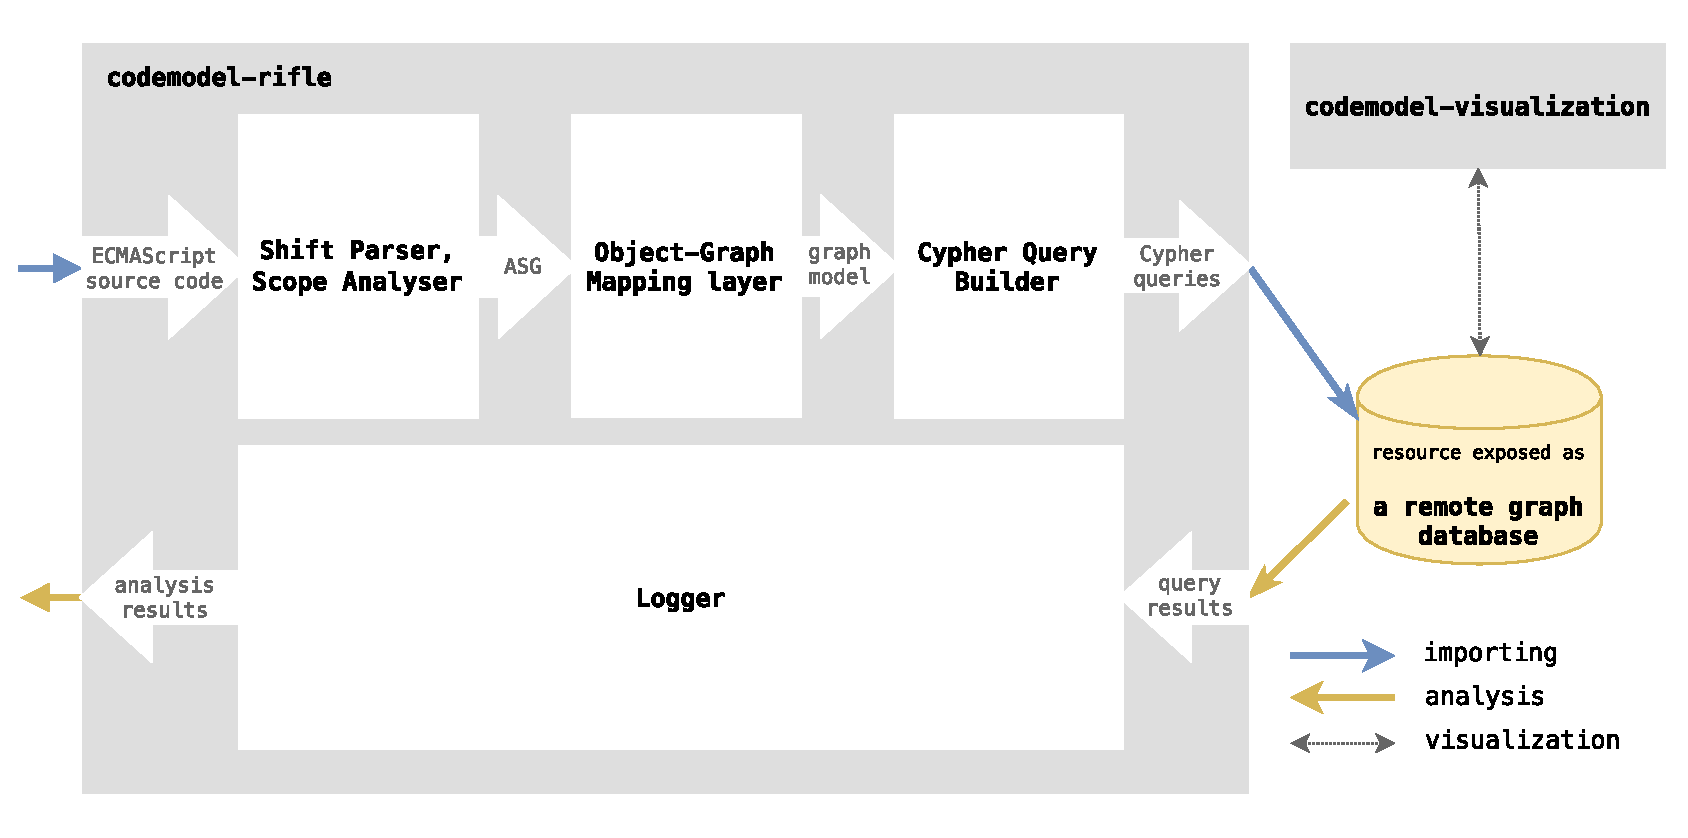
\includegraphics[width=\textwidth, trim=3mm 3mm 3mm 3mm,clip]{figures/codemodel-rifle-refactored-architecture.pdf}
	\caption{The refactored architecture of the Codemodel-Rifle framework}
	\label{fig:codemodel-rifle-refactored-architecture}
\end{figure}


\section{In Development: Steps of Building New Analyses}

Building new analyses to catch new software defects basically consists of three steps. The steps are detailed in the following subsections.


\subsection{Visualising the Defect with Codemodel-Visualisation}

First, the defect has to be inspected with the ASG-semantics of Codemodel-Rifle. For visualising a defect pattern, a new unit test has to be implemented in the Codemodel-Visualization project. The JavaScript module or modules containing the defect should be included as test resources.

Using Codemodel-Rifle as a dependency, Codemodel-Visualization first imports the file (files) and translates it (them) to separate property graphs. If multiple source files are imported, their graphs are connected along the export and import semantics of ECMAScript.\footnote{The process of connecting ECMAScript modules along export and import statements is one of the key subjects of this thesis. It will be detailed in Chapter 5.} Finally, the full property graph model gets exported into visual file format, like PDF or PNG.


\subsection{Describing the Defect Pattern}

The file exported by Codemodel-Visualization precisely mirrors the property graph instance model transformed by Codemodel-Rifle, but some nodes and edges are not displayed to preserve the transparency of the visualised graph.\footnote{Ignored nodes and edges are listed in the \texttt{GraphWalker} class as filtered entities from the underlying visitor pattern implementation.} Any pattern seen in the visualised graph can be directly matched by Codemodel-Rifle.


\subsection{Implementing the Analysis}

Analyses are basically Cypher queries. If a defect's pattern can be expressed with a Cypher query in some way, it can be detected by the framework.

Some defects are more high-level or more general than to present their patterns in an intact graph directly. Detecting complex errors like these may require to extensively manipulate the graph to dredge defect patterns for matching. In cases involving \emph{transitive} defects, like in the running example\footnote{The running example is to detect a division by zero scenario. But zero is not a numeric literal $0$, but the indirectly referenced return value of a nested function stack with variable assignments and also a module boundary in between.} presented in Chapter 2, a flag like \texttt{EqualsZero} has to be propagated through the graph along specified edges: variable assignments, variable references, function call and function return statements, etc.

Transitive graph manipulations can be achieved by introducing \emph{qualifiers} into the analysis. The concept of qualifiers will be described in detail in Chapter 5.

If the analysis matches the specified pattern, my implementation returns the following:

\begin{itemize}
\item a \textbf{message} to explain the type of the defect for a human reader,
\item an \textbf{entity name} (or an empty string) to identify defects bound to named entities,
\item the \textbf{path} of the containing module,
\item the \textbf{line} in which the defect was found,
\item the \textbf{column} of the line at which the defect begins.
\end{itemize}

In my current implementation, these items are uniformly\footnote{Exactly these items are returned in all cases, regardless of the defect type.} returned from the database as elements of a Neo4j \texttt{Record}, and they are handed over to a central logger to be immediately printed after minimal formatting. This is not a flexible, extensible solution; in the future, this basic defect processing logic should be refined. The found defects could be returned as JSON objects from the database to be represented as instances of the \texttt{Defect} Java class. They could also be collected into a per-analysis data structure. This way, the framework could display defects found at an analysis according to various aspects and criteria, and it could also produce machine-readable output for other software.


\section{In Production: Steps of Operating Live}

The prospective live operation of the framework basically consists of three steps, which are managed by the framework. Ideally, the operation should be automatic and transparent: if a change is done in the IDE, or a new commit is pushed to the central repository, the framework should perform an analysis over the changed code repository. The steps of a full analysis procedure are detailed in the following subsections.


\subsection{Synchronising the Repository into the Framework}

First, the code repository is imported into the framework. This involves listing and parsing all files with configured extensions (currently only \texttt{.js}), then saving the created property graph models into the database.

The word synchronising expresses that Codemodel-Rifle aims to be incremental; but while it does so, its capabilities are still very limited. According to plans, the framework will cooperate with VCSs to detect changes, thus it will be able to import only those files that changed since the last import process.


\subsection{Connecting the Related ECMAScript Modules}

To evaluate analyses over multiple ECMAScript modules, the related modules' separate property graphs are interconnected along the export and import semantics of ECMAScript. This process is described in detail in Chapter 5.


\subsection{Performing Analyses}

Performing analyses can be broken down into two substeps.


\subsubsection{Manipulating the Graph}

Complex analyses may require to extensively manipulate the graph. These manipulations involving qualifiers are processed first.


\subsubsection{Querying the Graph}

The graph is queried with Cypher, with matching predefined graph patterns developed with the aforementioned steps. If a defect pattern matches, the defect gets logged onto the console in the format seen in \Cref{fig:defect-found-logger}.

\vspace{0.5em}
\begin{figure}[!htb]
	\centering
	\texttt{\textbf{message}: \textbf{entityname} at \textbf{line}:\textbf{column} in \textbf{path}}
  \caption{The framework's console output if a defect was found}
  \label{fig:defect-found-logger}
\end{figure}